\chapter{Software Implementation}\label{chap:3}
Now that we have all the theoretical and practical elements of the system, here we report all the work done to implement it on a software side. That includes code written from scratch and also code used to interface with already existing parts. This chapter can be divided in 4 parts:
\begin{enumerate}
    \item introduction of all the basics libraries used;
    \item description of the code implemented to control the turret and the solution adopted to overcome the issues mentioned in \ref{subs:firstModel:issues};
    \item explanation on how we interface with the arm pointing system and the relative localization procedure;
    \item demos implementation.
\end{enumerate}
Experiment setups and procedures are left for chapter \ref{chap:4}.

\section{Libraries and Frameworks}
The system developed is composed by many modules handling different functionalities. It is worth to mention a couples of libraries and frameworks which are widely used throughout the project, as some of them are also primary to understand the implementation. In the next section we will give an overview of:
\begin{itemize}
	\item \ac{ROS} Kinetic Kame
	\subitem \texttt{rospy} 1.12.13
	\subitem \texttt{rosbag} 1.12.13
	\subitem \texttt{tf} 1.11.9
	\item \texttt{Dynamixel Workbench} and \texttt{Dynamixel SDK}
	\item \texttt{NumPy} 1.14.3
	\item \textttt{Matplotlib} 2.2.2
	\item \texttt{pandas} 0.23.0
\end{itemize}
The programming language used for development is Python 2.7.12.\\

\subsection{\acf{ROS}}
\ac{ROS} is a open-source\footnote{Main client libraries and tools are under the terms of the BSD license (\url{https://en.wikipedia.org/wiki/BSD_licenses}).} meta-operating system for robots \cite{ros}. \ac{ROS} is the industry and research standard framework for robotics and it is aimed to help software developers to  create robotic applications.\\

Its primary goal is to support code reuse in robotics research and development. \ac{ROS} is a distributed framework of processes (aka Nodes) that enables executables to be individually designed and loosely coupled at runtime. These processes can be grouped into Packages and Stacks, which can be easily shared and distributed. \ac{ROS} also supports a federated system of code Repositories that enable collaboration to be distributed as well. This design, from the filesystem level to the community level, enables independent decisions about development and implementation, but all can be brought together with \ac{ROS} infrastructure tools.\\
At the lowest level, ROS offers a message passing interface that provides inter-process communication and is commonly referred to as a middleware.
The ROS middleware provides these facilities \cite{ros:core-components}:
\begin{itemize}
    \item publish/subscribe anonymous message passing
    \item recording and playback of messages
    \item request/response remote procedure calls
    \item distributed parameter system
\end{itemize}
In addition to the core middleware components, ROS provides common robot-specific libraries and tools to get a robot up and running quickly. Here are just a few of the robot-specific capabilities that ROS provides:
\begin{itemize}
    \item Standard Message Definitions for Robots
    \item Robot Geometry Library
    \item Robot Description Language
    \item Pose Estimation
    \item Localization
    \item Mapping
    \item Navigation
\end{itemize}
in particular, the \emph{Robot Geometry Library} is widely used for that project.
\subsubsection*{Robot Geometry Library: tf}
A common challenge in many robotics projects is keeping track of where different parts of the robot are with respect to each other. For example, if one wants to combine data from a camera with data from a laser, he needs to know where each sensor is, in some common frame of reference. This issue is especially important for humanoid robots with many moving parts. This problem is addressed in ROS with the \texttt{tf} (transform) library, which will keep track of where everything is in the robot system.

Designed with efficiency in mind, the \texttt{tf} library has been used to manage coordinate transform data for robots with more than one hundred degrees of freedom and update rates of hundreds of Hertz. The \texttt{tf} library allows one to define both static transforms, such as a camera that is fixed to a mobile base, and dynamic transforms, such as a joint in a robot arm. One can transform sensor data between any pair of coordinate frames in the system. The \texttt{tf} library handles the fact that the producers and consumers of this information may be distributed across the network, and the fact that the information is updated at varying rates.\\
\texttt{tf} lets the user keep track of multiple coordinate frames over time. \texttt{tf} maintains the relationship between coordinate frames in a tree structure buffered in time, and lets the user transform points, vectors, etc between any two coordinate frames at any desired point in time.

\subsubsection*{Nodes}
\ac{ROS} nodes are executable files that use \ac{ROS} to communicate with other nodes. Nodes are usually fine grained processes that perform precise computations. To communicate, nodes use a ROS client library to publish or subscribe to \emph{topics} or \emph{services}. Different Nodes can run on different hardware while being in the same \ac{ROS} system.

\subsubsection*{Bags}
Another function of \ac{ROS}, are \lstinline|rosbag| files. Bags are a format for saving and playing back ROS message data. Bags are an important mechanism for storing data, such as sensor data, that can be difficult to collect but is necessary for developing and testing algorithms.


\subsection{Dynamixel SKD}
The \texttt{ROBOTIS Dynamixel SDK} is a software development kit that provides Dynamixel control functions using packet communication. The API of Dynamixel SDK is designed for Dynamixel actuators and Dynamixel-based platforms. It is based on C/C++ programming. The Dynamixel SDK supports all Dynamixel series developed by \texttt{ROBOTIS}. For example, all series such as AX, RX, EX, MX, XL, XM, XH, PRO-L, PRO-M and PRO-H are supported by packet communication.
\begin{figure}
	\centering
	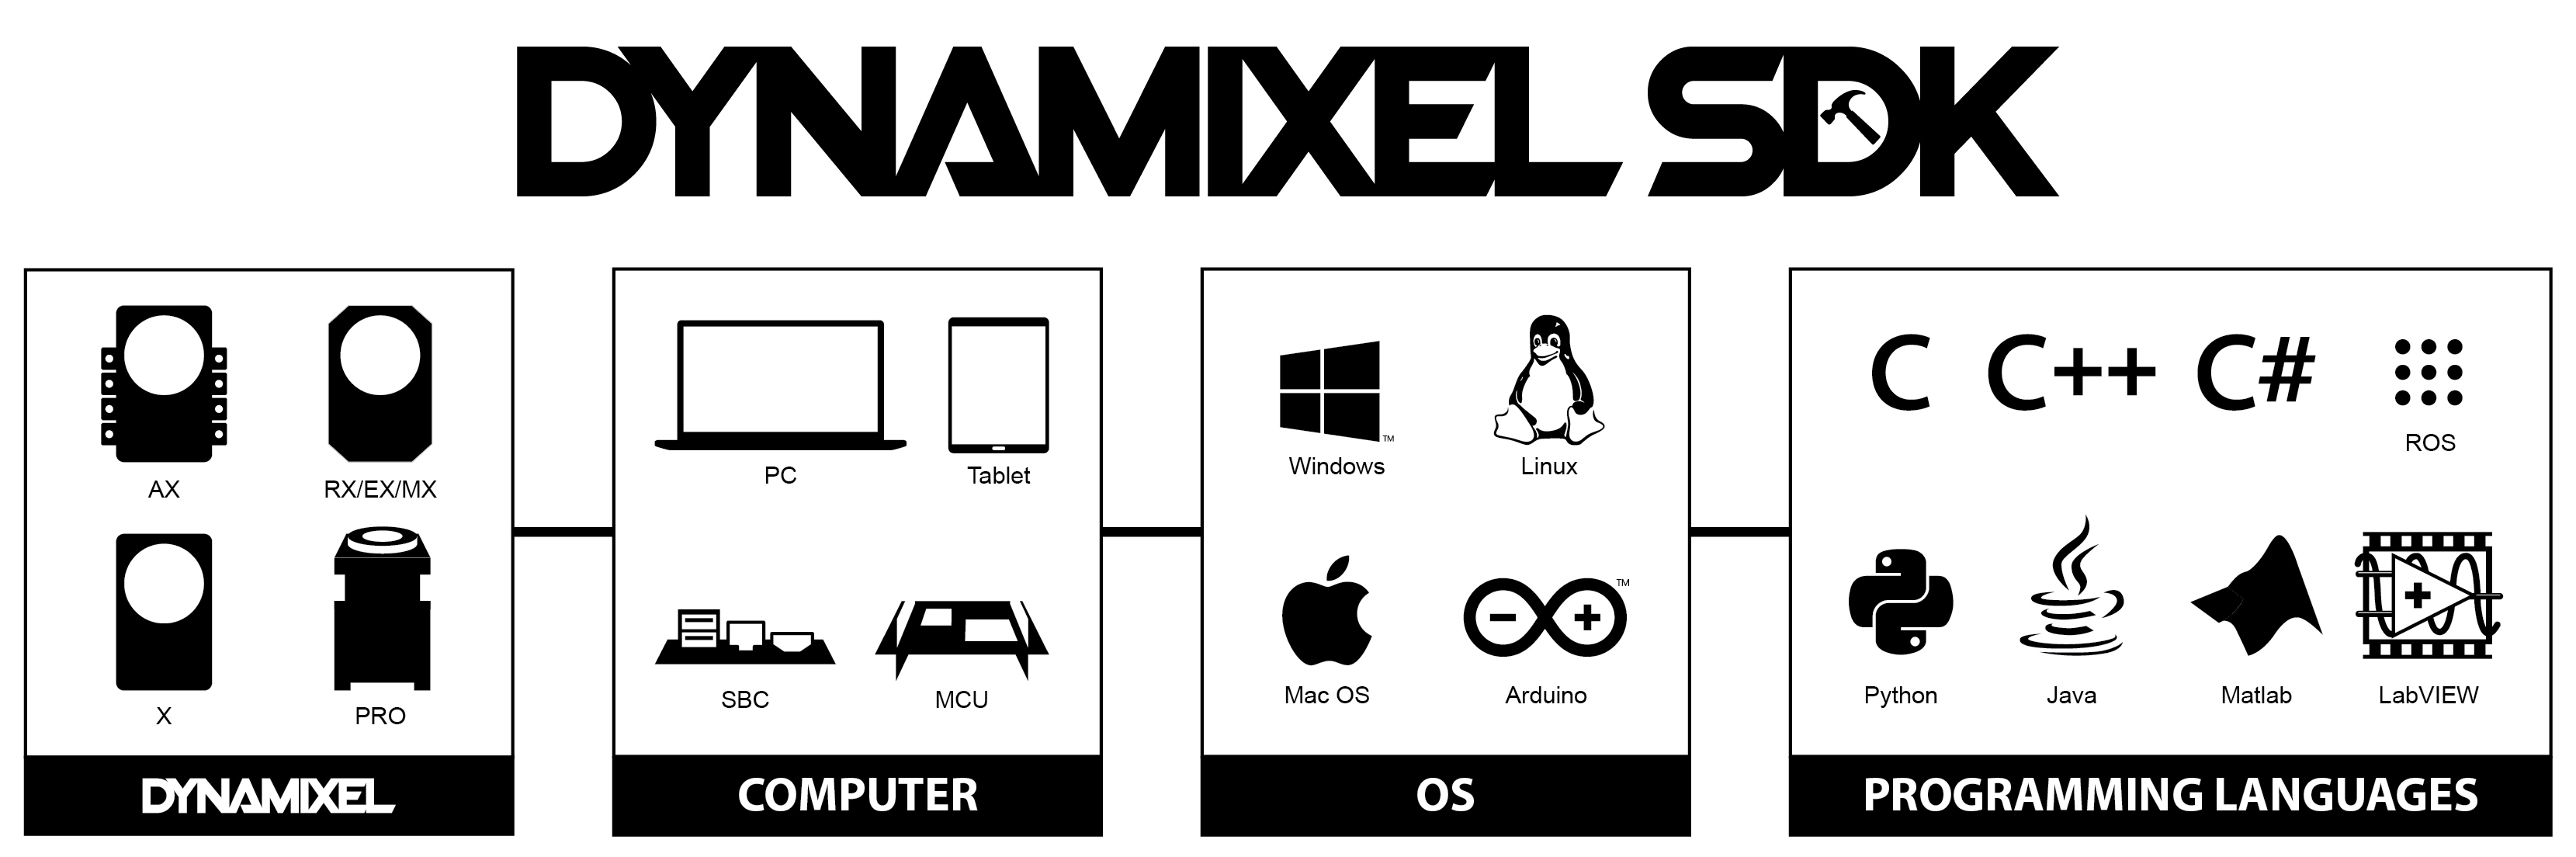
\includegraphics[width=\textwidth]{img/sdk.jpg}%
	\caption{Dynamixel SDK}
	\label{fig:turretPipeline}
\end{figure}

\subsection{Dynamixel Workbench}
Dynamixel-Workbench is dynamixel solution for ROS. This metapackage allows one to easily change the ID, baudrate and operating mode of the Dynamixel. Furthermore, it supports various controllers based on operating mode and Dynamixel SDK. These controllers are commanded by operators.


\subsection{Numpy}
NumPy is the fundamental package for scientific computing with Python \cite{numpy}. It contains among other things:
\begin{itemize}
    \item a powerful N-dimensional array object
    \item sophisticated (broadcasting) functions
    \item tools for integrating C/C++ and Fortran code
    \item useful linear algebra, Fourier transform, and random number capabilities
\end{itemize}

Besides its obvious scientific uses, NumPy can also be used as an efficient multi-dimensional container of generic data. Arbitrary data-types can be defined. This allows NumPy to seamlessly and speedily integrate with a wide variety of databases.
\subsection{Matplotlib}
Matplotlib is a Python 2D plotting library which produces publication quality figures in a variety of hardcopy formats and interactive environments across platforms \cite{matplotlib}. Matplotlib can be used in Python scripts, the Python and IPython shells, the Jupyter notebook, web application servers, and four graphical user interface toolkits.\\

Matplotlib makes plotting high quality graphs accessible to anyone. With Matplotlib it is possible to generate a wide variety of types of plots from histograms to scatter plots with just a few lines of code.\\

Matplotlib tries to make easy things easy and hard things possible. One can generate plots, histograms, power spectra, bar charts, errorcharts, scatterplots, etc., with just a few lines of code. 
Matplotlib uses a MATLAB-like interface. Power user have full control of line styles, font properties, axes properties, etc, via an object oriented interface or via a set of functions similar to MATLAB one.
\subsection{pandas}
\label{sec:pandas}
pandas\footnote{The name is written in lowercase letters.} is an open source community supported, BSD-licensed library providing high-performance, easy-to-use data structures and data analysis tools for Python. pandas is still in active development and since it has seen a growth in adoption, on the official documentation multiple guides are present to help shifting from another environment or language like R.

\section{Turret Software Implementation}
First, we must recall what are our goals. We want to be able to drive a laser dot on a given surface (i.e. the floor) by setting its \emph{x} and \emph{y} coordinates (the \emph{z} would be implicit on the floor). This must be done with a good precision and also with high frequency, as we want to draw nice and smooth trajectories with the laser. To do so, we can only control two Dynamixel servos, setting their angles values accordingly to the inverse kinematics solved in \ref{sec:1.1}.\\
So, we will describe how we implement the turret model and then the interface written to control the motors and achieve our goals.
\subsection{Turret Model Implementation}
The two turret models are implemented as ROS node containing the inverse kinematic equation and the code to publish the \texttt{tf tree} of the turret. Those models, in fact, are simply implemented as a chain of \texttt{tf frames}. In that way, we can easily keep track of the position/transformation of our frame, corresponding to our \emph{pan} and \emph{tilt} angle. This is an immediate implementation of the logic already depicted in figures \ref{fig:firstModelRefFrame} and \ref{fig:secondModelRefFrame}.\\
So, those are the nodes in charge to compute and keep track of the values of our two DoF.


\subsection{Motors Controller}
The drivers for both the AX-12+ and the MX-64 Dynamixels are provided by the \texttt{dynamixel sdk}. Moreover, the \texttt{dynamixel workbench} offers ROS interfaces to work with the official sdk. That is one of the most crucial part of software, because it is directly related to the issues mentioned in section \ref{subs:firstModel:issues}. As a matter of fact, it is where we intervene to solve those issues, which are mostly due to the slow communication protocol. As a matter of fact, we motors are not able to process all the points composing the trajectory that we need to send at 50Hz and they simply drop them. That happens because each time a command is sent through the bus interface, each motors has to reply with an acknowledgment. So, we disable all kind of response from the servos, assuming that once a command is sent, it will be properly executed. Moreover, we hack the drivers to be sure that the PC will not wait for motors replies. That is a bit tricky as, even though the low level function to write the servos registries without wait for reply exists, we have to find and expose it through the workbench libraries.\\
Given that, we are able to draw our smooth trajectories in the simplest way possible: sending points at a fixed rate with the servos in joint mode. \emph{Joint mode} means \emph{position control}. In other word, we can directly specify the value of the position/angle we want the servo to reach to the servo itself. Its internal controller will move the motor accordingly.\\
That works fine with the first turret model, but also with the second one. Even better, the \emph{MX-64} based turret works perfectly thanks to its better servo resolution.\\

Even if the two turret model could use the same interface, the software project contains two different ones as, for the first turret, we use an unofficial low level driver that is tightly coupled with the architecture of the Dynamixel \emph{AX-12+} itself and thus is not reusable. On the contrary, for the second turret, the code is rewritten to directly exploit the generic ROS service interface offered by the \texttt{dynamixel workbench}. That code would also work with the first model.\\
Finally, we have a useful module to publish the points composing the desired trajectory.

\subsection{Laser Turret Complete Picture}
Now that all the software parts composing the turret have been introduced, we can put everything together to understand exactly how the code is modulated and which module is in charge of what. Here we will consider the file related to the \emph{MX-64} turret. Figure \ref{fig:turretPipeline} give us an idea.
\paragraph{tf\_broadcaster} is the module containing and simulating the geometrical model of the turret. It also computes the inverse kinematic of the laser dot. So, this is the piece of software in charge of computing the joints position (i.e. \emph{pan} and \emph{tilt} values) corresponding to the laser dot goal position (expressed in the reference frame of the turret). It only takes a 3D point as input, but serves all our purposes: it can be used to draw a trajectory, as long as ones send a stream of point as input; it can be used to follow the human pointing, after the relative localization is done; it can, of course, mark a single spot on the floor (as we need it for the experiments).
It will publish those values and update its internal representation of the turret accordingly, but it will not directly send the commands to move the motors. This is very convenient, as it allows us to simulate the system even without a physical turret and decouples the logical model from the physical controller.\\
\paragraph{turret} module contains that physical controller. Again, that code is written with the idea of making the system modular. In fact, this class leverages on the \texttt{dynamixel workbench} to send commands to any Dynamixel motors. In that way, as long as we are working with a device which needs to set only two angles (e.g. \emph{pan} and \emph{tilt} unit), we can plug into the system any turret built with any Dynamixel motor model. Needless to say, that was helpful when we had to deal with two different turret models.\\
\paragraph{trajectory\_publisher} is needed to decide the shape of the trajectory to draw. Then, it will publish each point at a fixed rate to the interface provided by \texttt{tf\_broadcaster}. In that way, the laser dot will follow the desired trajectory. We can draw many different shapes, but in our experiments and demos we use the \virgolette{$\infty$} shape.

\begin{figure}
	\centering
	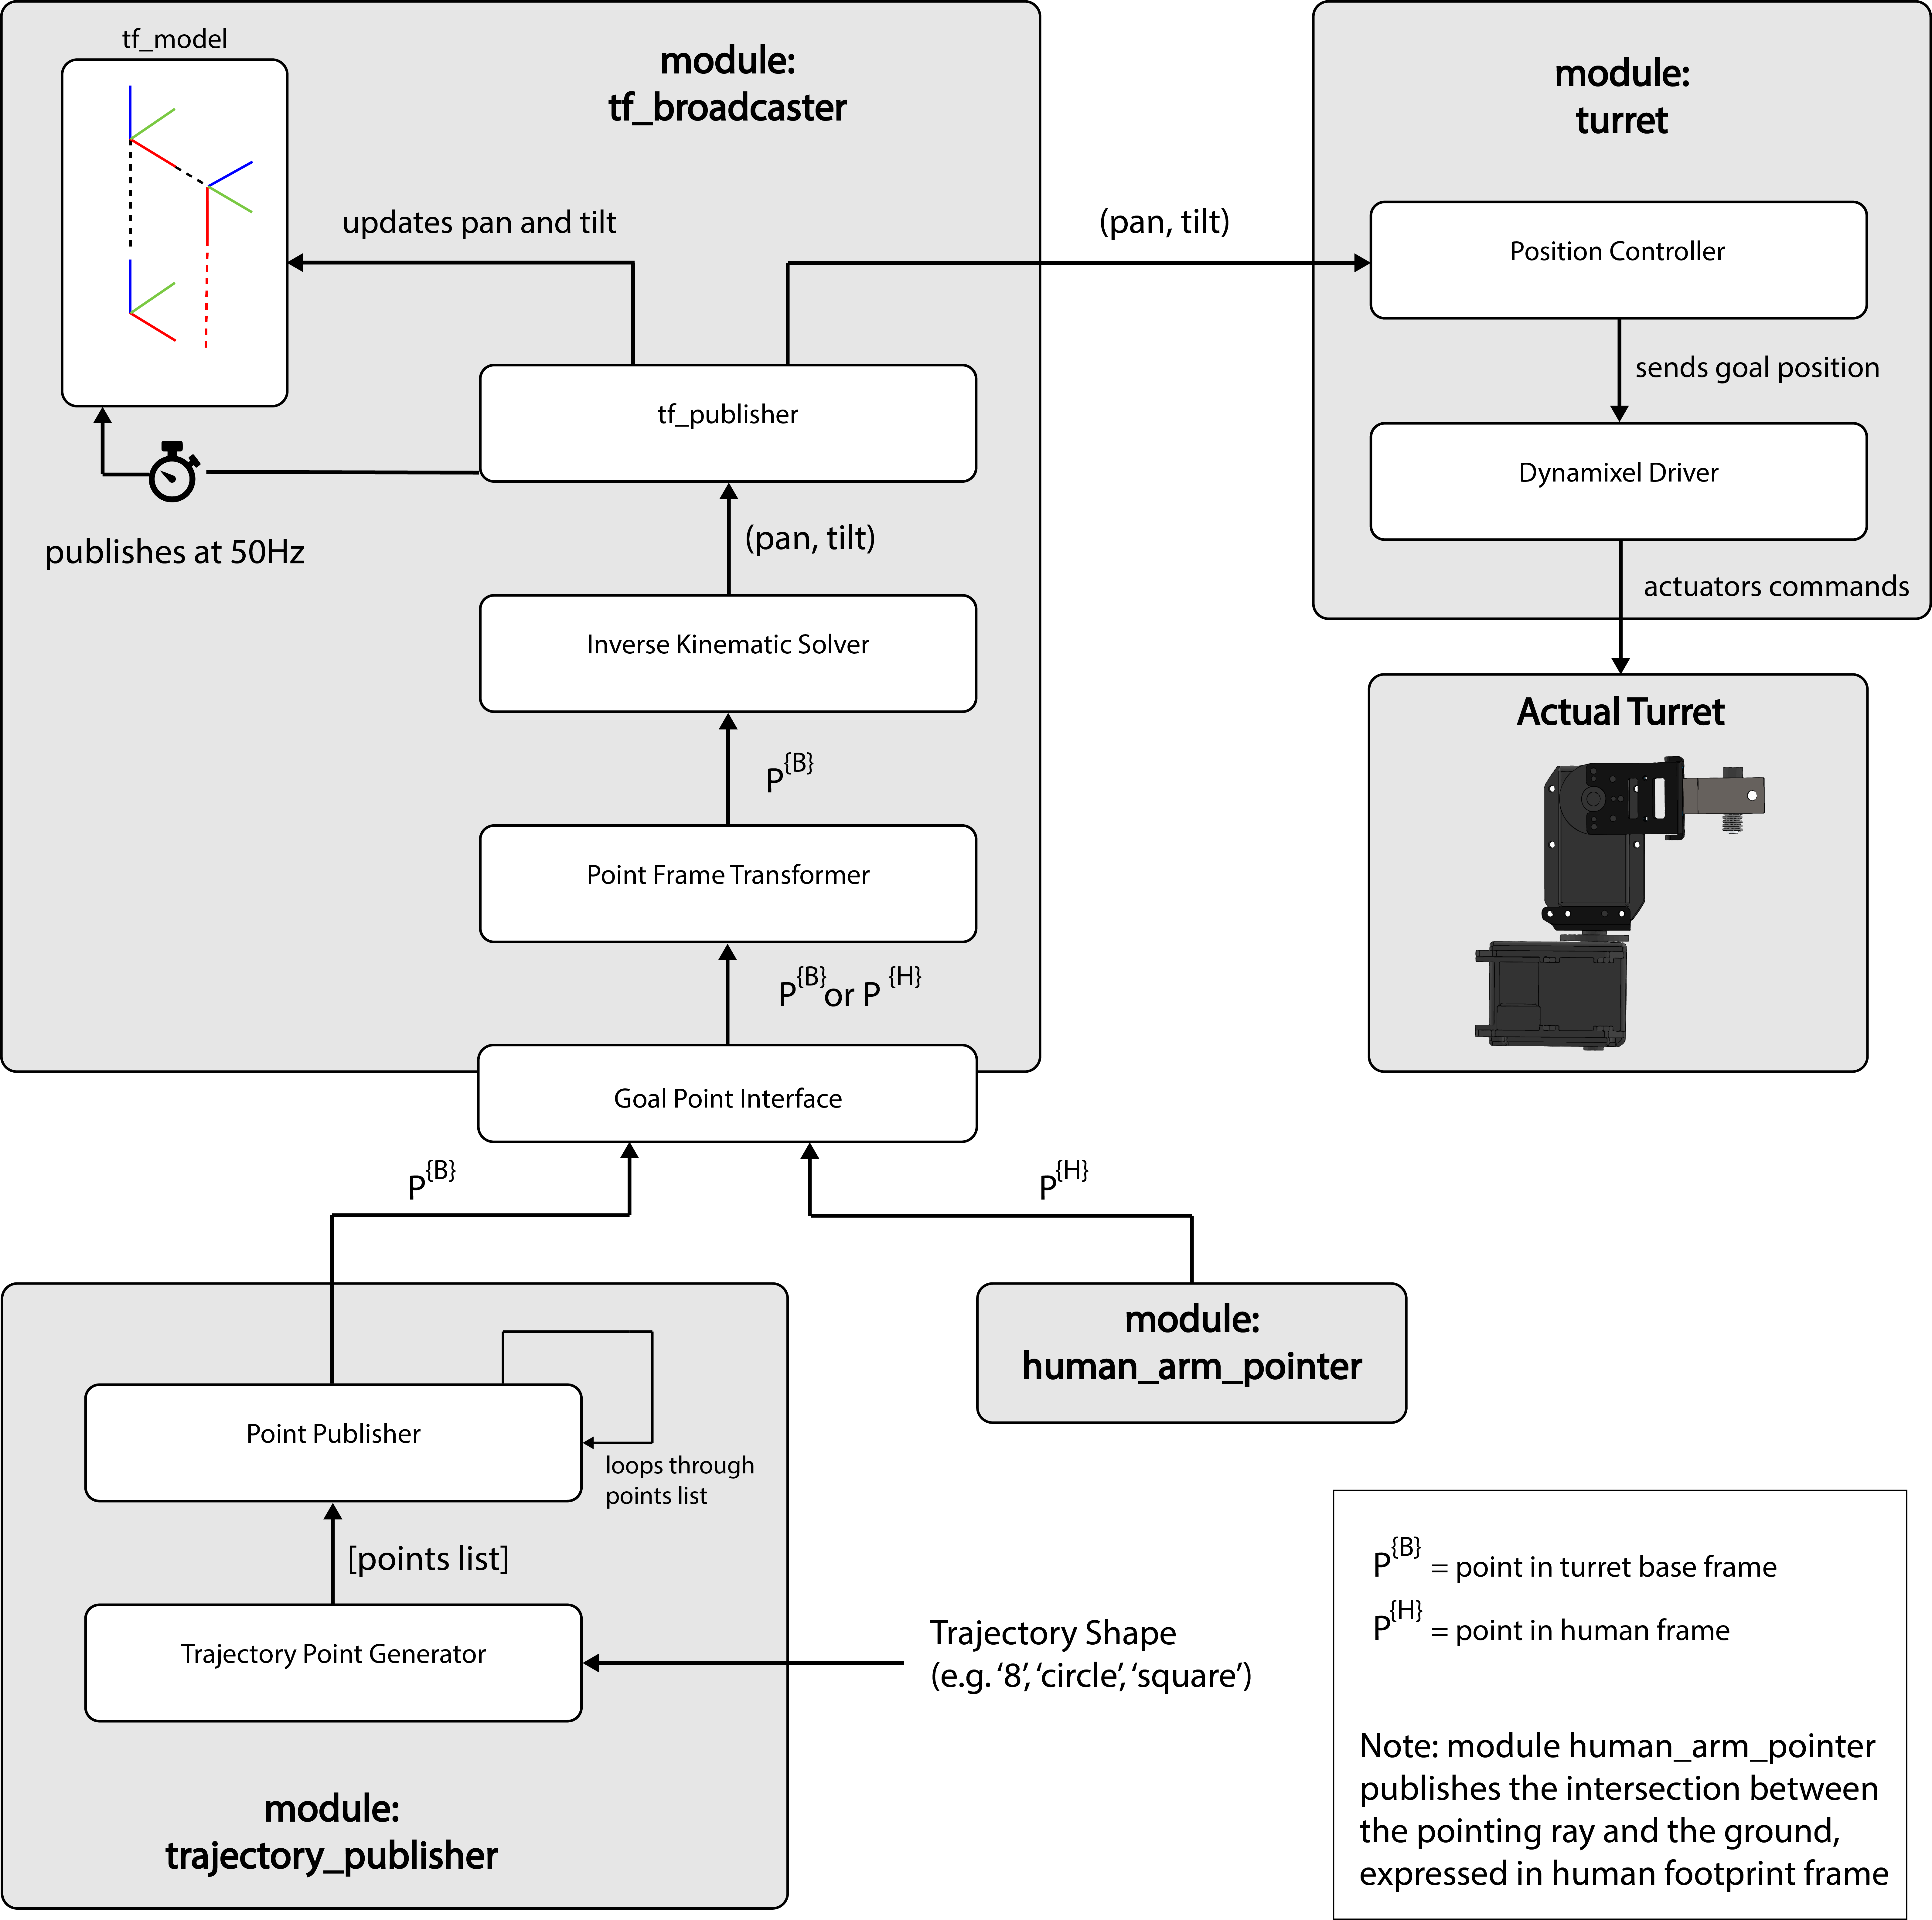
\includegraphics[width=\textwidth]{img/turretPipeline.png}%
	\caption{Laser Turret Implementation, the Complete Picture}
	\label{fig:turretPipeline}
\end{figure}


\section{Pointing Software Implementation}
As explained in section \ref{sec:1.2}, we are using the human pointing model suggested and implemented for \cite{gromov2018robot}. The geometry already presented in that section is very convenient as it can be implemented directly into code, as in the \textbf{arm\_node} module.\\
Thus, is very simple to understand how that part works: we receive as input the quaternions (i.e. the rotation) from the wearable IMU. In that way we can determine the direction of the pointing ray that we know has its origin between the eyes and passes through the fingertip of the human, exactly as previously shown in figure \ref{fig:pointingModel}. That requires also that certain measures of users' bodies are known. In particular, for each user we take the height which goes from the ground to the centroid of the head, from the shoulder to the wrist and from the wrist to the fingertip\\ 
We will not explain that code in details since it was not developed for that thesis, but we will mention one interesting fact related to pointing on the floor and the differences occurred when implementing the pointing on the wall (that part was developed for the thesis).
\subsection{Pointing on the Floor}
Keeping in mind that the pointing ray is an infinite line, we can easily see that there is a problem: when the human is pointing above the horizon (i.e. is not pointing on the floor), the ray will be still intersecting the plane behind the human. Luckily, for how things have been defined in \ref{eq:intersection}, we can simply check whether $s_I \geq 1$ to be sure that the intersection is ahead of the human. If not (also if the ray is parallel to the floor), we do not have a valid intersection, thus we return a pose for the human made with \texttt{NaN} values.
\subsection{Floor vs Wall}
As already stated, for that thesis we implemented also a demo with the user pointing on the wall. The implementation for the pointing itself was pretty straightforward, as it is similar to the one on the floor, but there are a couple of details that are implicit when pointing on the floor and that must be taken into account for the wall case. In fact, assuming that the human is standing on a flat plane perpendicular to him, which is a fair assumption for our system, we already know the distance from the floor (i.e. $0$) and its orientation. So, we know that if the human is not pointing above the horizon, we have an intersection. However, in the wall case, we have to explicitly know and set the distance of the human from the wall and its orientation to intersect the pointing ray. That makes the demo for our system on the wall limited by those initial conditions that, on the contrary, can be implicitly taken for granted in the floor case.


\section{Relative Localization Software Implementation}
As for the the pointing, the relative localization (relloc) implementation is the same proposed in \cite{gromov2018robot}. However, that code was written to work with a drone, so a flying robot with an odometry which is slightly different from a ground robot (and a laser point). For that thesis, only a couple of modifications were needed to interface the turret and then replace the drone with the laser dot. The result can be seen in \textbf{motion\_relloc} module. In that section we will give an overview of how that procedure is implemented in terms of input and output.
\subsection{Relloc Input}
As already explained in \ref{sec:relloc}, the relloc procedure takes as input a set of pairs composed by the position of the laser dot in the turret frame and the \emph{corresponding} pointing ray in human frame. \emph{Corresponding} means that we want to get the data of the ray generated by the human while the turret was marking that particular point with the laser. This is crucial, because it means that data must be synchronized precisely. This also explains why we wanted the turret to be  as precise, fast and smooth as possible. Thus, we are sending trajectory point to the turret at $50 Hz$ and collecting data from the arm IMU at the same rate.\\
To build our input set we specify the duration of the interaction in seconds (usually is $5s$ in our demos) and the number of pairs to sample (usually $250$). Since in $5$ seconds at $50 Hz$ we collect exactly $250$ pairs, it means that we usually sample the whole set. We use those values as $5$ second are enough to draw an $\infty$ shaped trajectory with a speed that allows the human to follow the laser easily.
\subsection{Relloc Output}
Recalling what was written in section \ref{sec:relloc}, the output of the relloc is the transformation:
\begin{align}
	\rho = [t_x, t_y, t_z, \gamma_z] \nonumber
\end{align}
which allows us to collocate the turret's frame pose (position and orientation) into the human's frame.\\
To obtain that transformation we iteratively call the optimization procedure contained already explained. We start with an arbitrary initial guess of:
\begin{align}
	\rho = [0, 0, 0, 0] \nonumber
\end{align}
and then try to reduce the error as defined in equation \ref{eq:error}, by sampling each pairs in a random order and updating $\rho$ accordingly.\\
In the end, we publish the transform of the turret into the human frame for a fixed time window (usually $60s$), leveraging on the functions provided by \texttt{tf}.
\section{System Complete Pipeline}
Now we finally have all the elements to understand the entire system pipeline, from the turret to the relloc. Figure \ref{fig:systemBigPicture} shows a schematic with all the involved modules. We can see that the turret draws a trajectory, the human follows that trajectory with pointing gestures. The system then puts together each laser point with each pointing ray and computes the relative localization. Once the relloc is estimated, it can be used for different applications, as we show with demos and experiments.
\begin{figure}
	\centering
	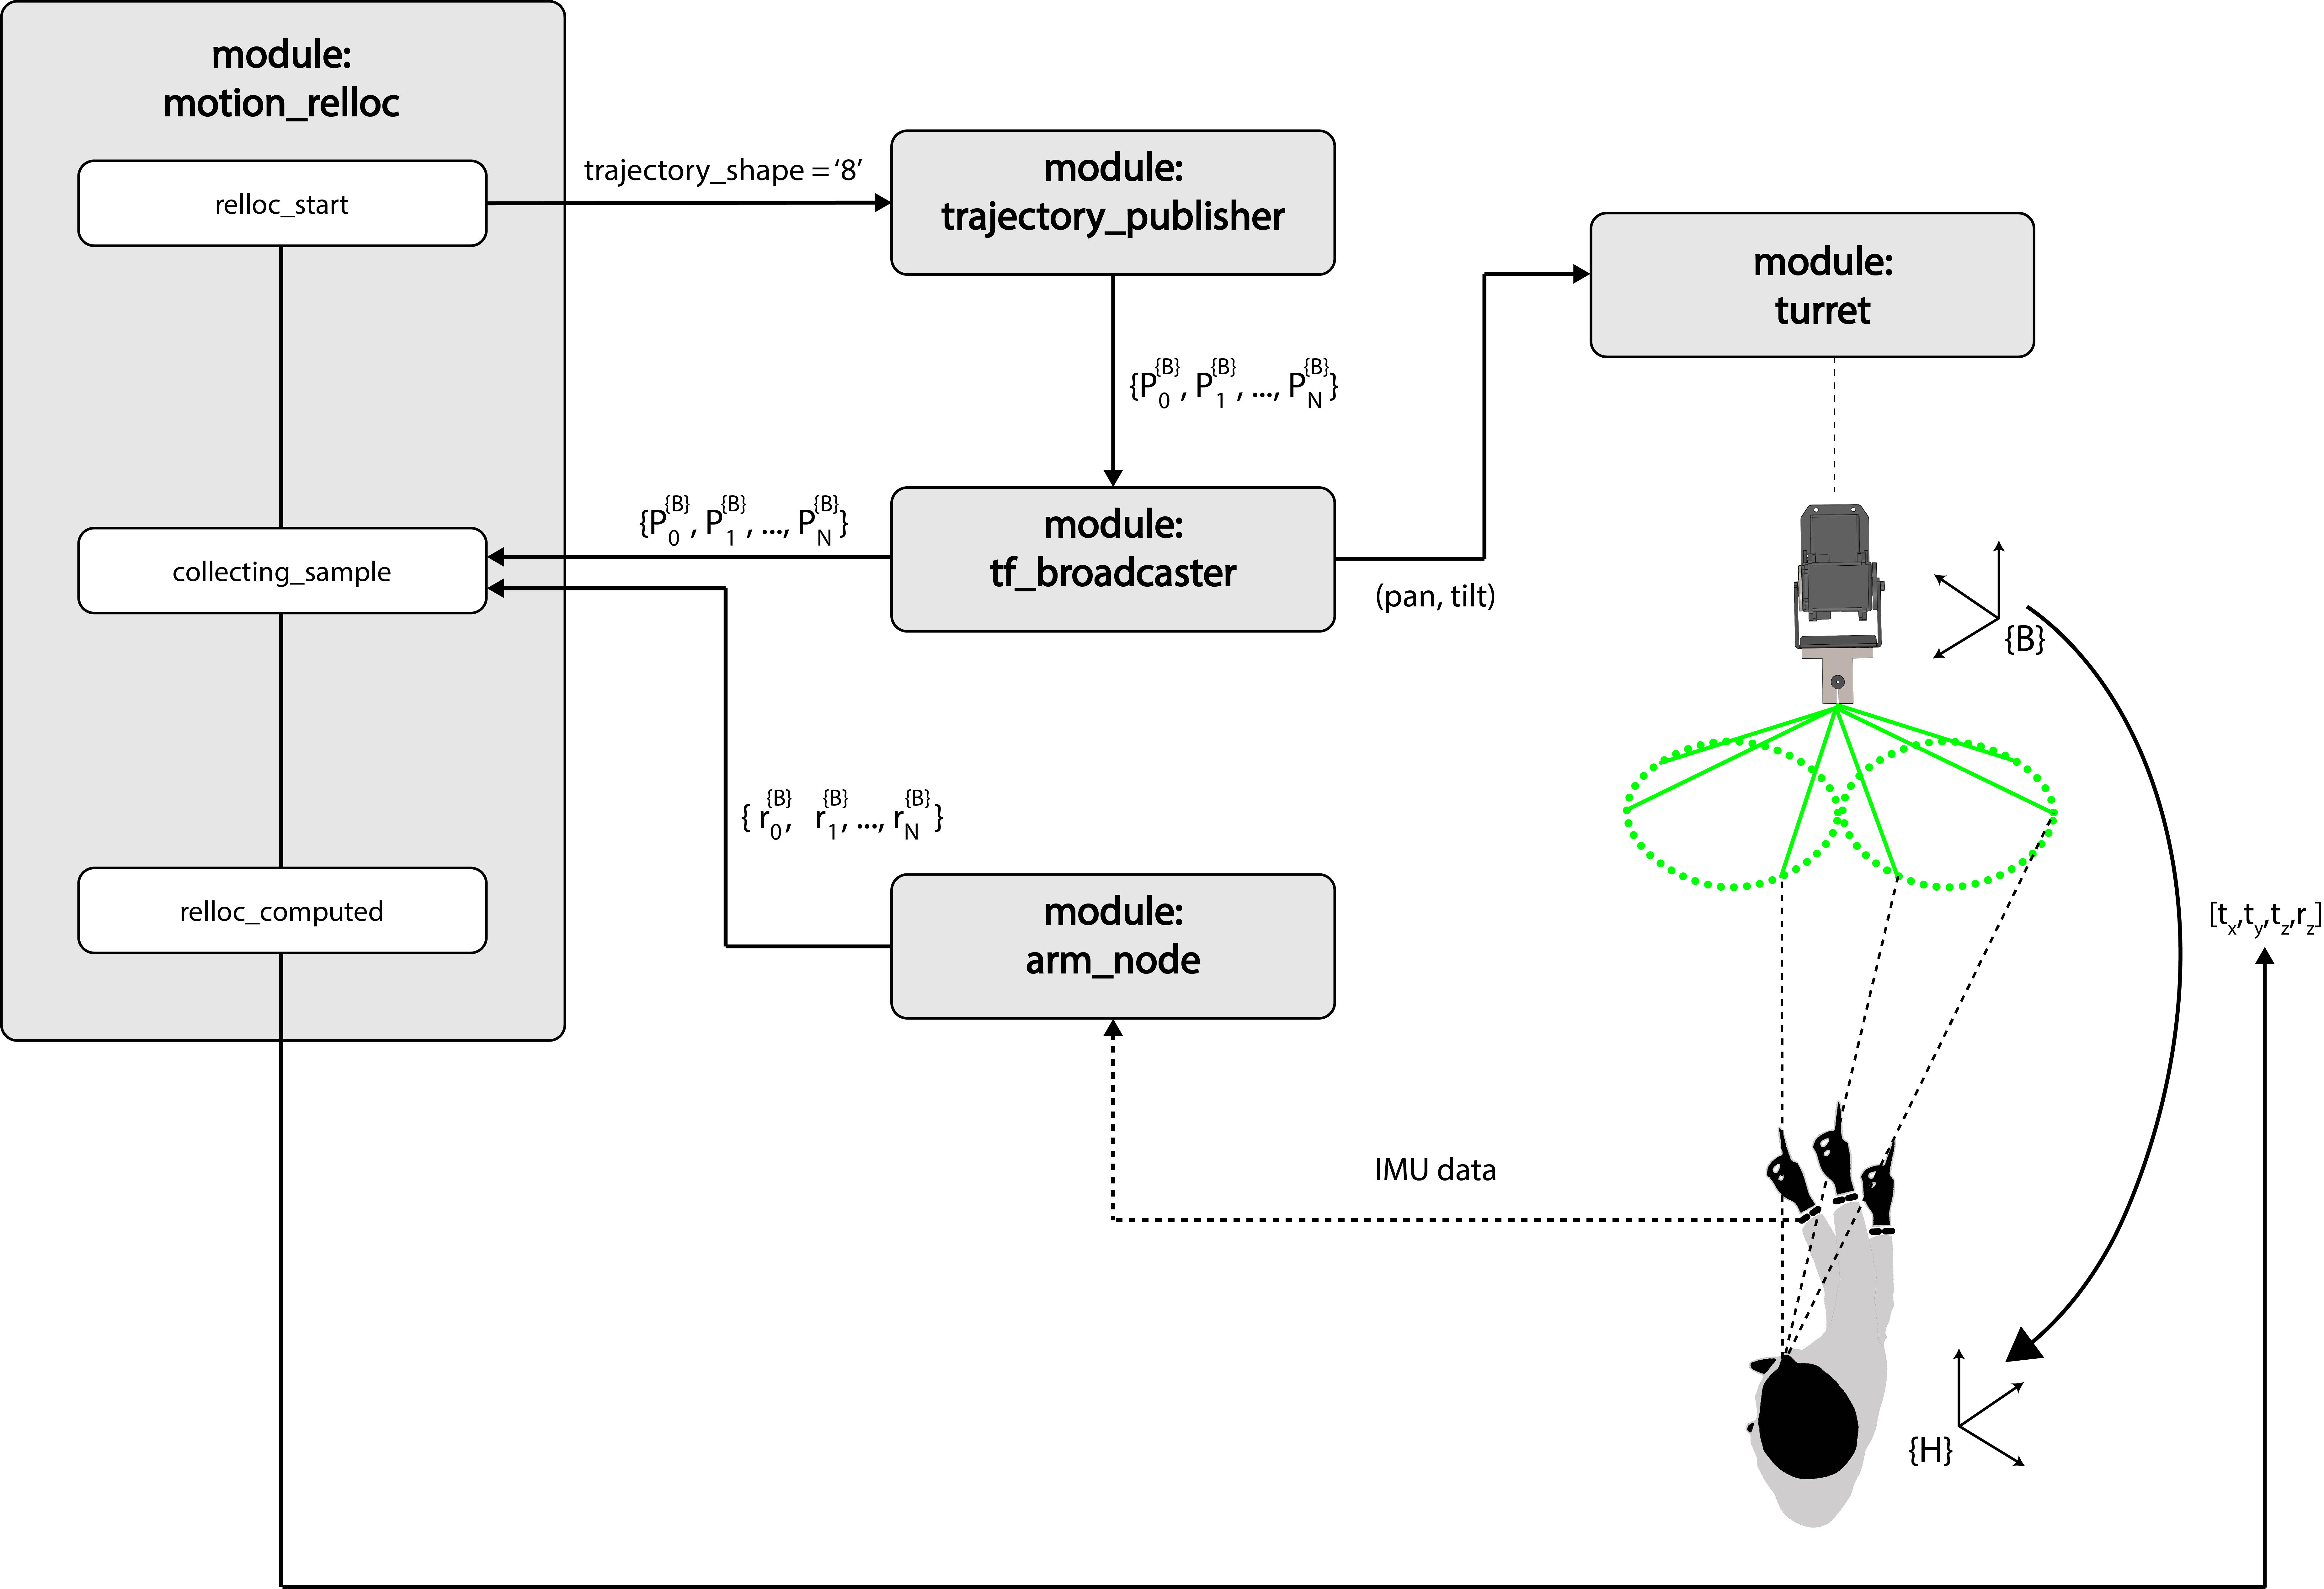
\includegraphics[width=\textwidth]{img/systemPipeline.png}%
	\caption{System Complete Pipeline}
	\label{fig:systemBigPicture}
\end{figure}

\section{Demos Implementation}
We have implemented three different demos to show the behaviour of the system and also demonstrate possible use cases. In that section we will discuss only aspects related to the software implementation of those demos. They are presented in depth in \ref{chap:4} 
\subsection{Relloc Demos}
Obviously, those demos are needed to give an example of the relloc. There are 2 different version of it. In both cases, first we compute the relloc, then we have two different behaviour: in one case, we use the estimated position to mark the point where the user is standing with the laser; in the other case, we allow the user to directly control the laser dot position on the floor (we implemented also a wall version) with pointing gestures.\\
In both cases, all we have to do is compute transformation between human and turret frame: in one case just to obtain the human position in the turret frame, in the other to obtain the point the human is pointing in the turret frame. All these transformations needed are easily obtained, as usual, thanks to the \texttt{tf} library for ROS, which played a major role for those demos. As a matter of fact, in figure \ref{fig:rellocDemo} we can see a user driving the laser around pointing at the ground. Since the relative location is known, goal points expressed with pointing rays in frame $\{H\}$ can be transformed into $\{B\}$ reference and thus be used to drive the turret.

To sum up, the module \textbf{relloc\_try} is taking care of all those transformations and easily interfaces itself with our core system.
\begin{figure}
	\centering
	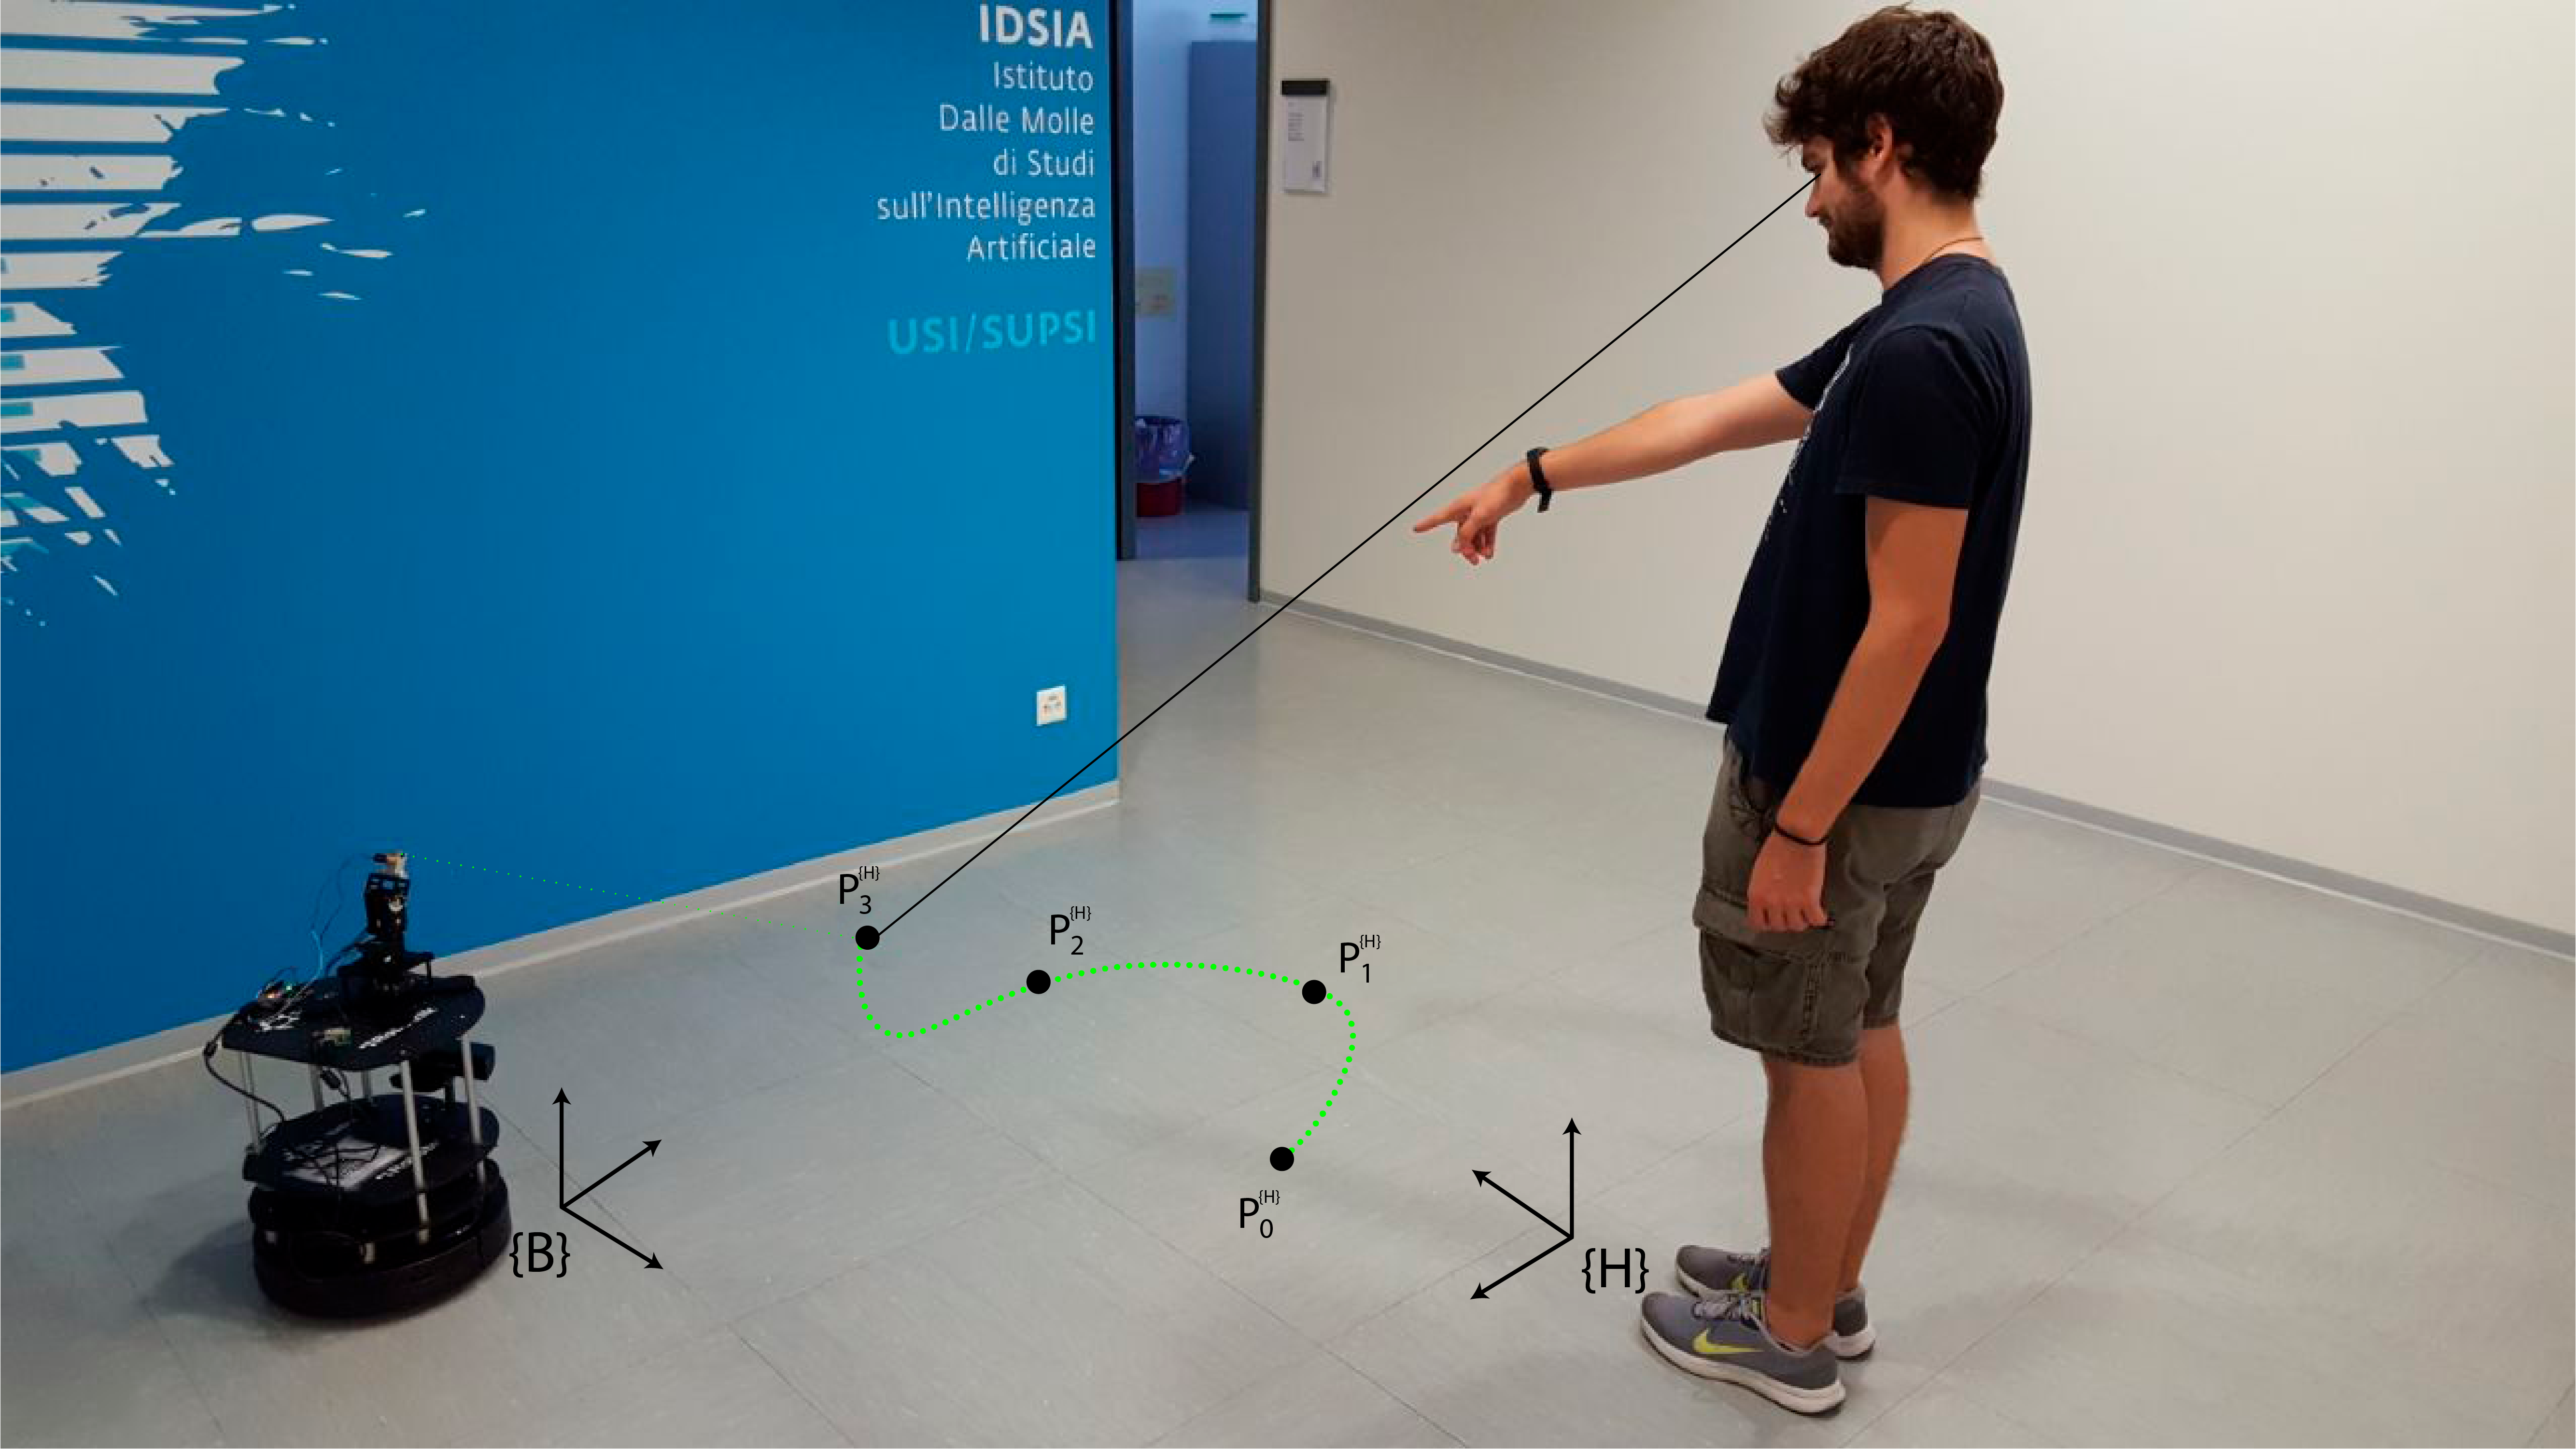
\includegraphics[width=\textwidth]{img/rellocDemo.png}%
	\caption{User Trying the Relloc Demo}
	\label{fig:rellocDemo}
\end{figure}
\subsection{Kobuki Go to Goal Demo}\label{subs:kobukiGoToGoal}
That demo exploits the kobuki platform to show an interesting use case for the system: mobile robot navigation.\\
In that case, we do the relloc and then tell the kobuki to reach a certain position by pointing at it for three seconds.\\
In addition to the relloc system, we implemented a basic PID controller to move the kobuki. The library to interface with the robot is available online \cite{kobuki:ROS}.\\ Moreover, To detect the fact that the user is pointing the same point for three seconds, we implemented a nice function with a fixed size queue where we store the coordinates of the last 150 laser points (which means points in the last $3$ seconds at $50Hz$). We check if the average distance of each point from the first point in the queue is within a given threshold: in that case we detect the 3 seconds pointing.\\
All that additional code is contained in the \textbf{kobuki\_go\_to\_goal} module, which interfaces flawlessly with our system.
\begin{figure}
	\centering
	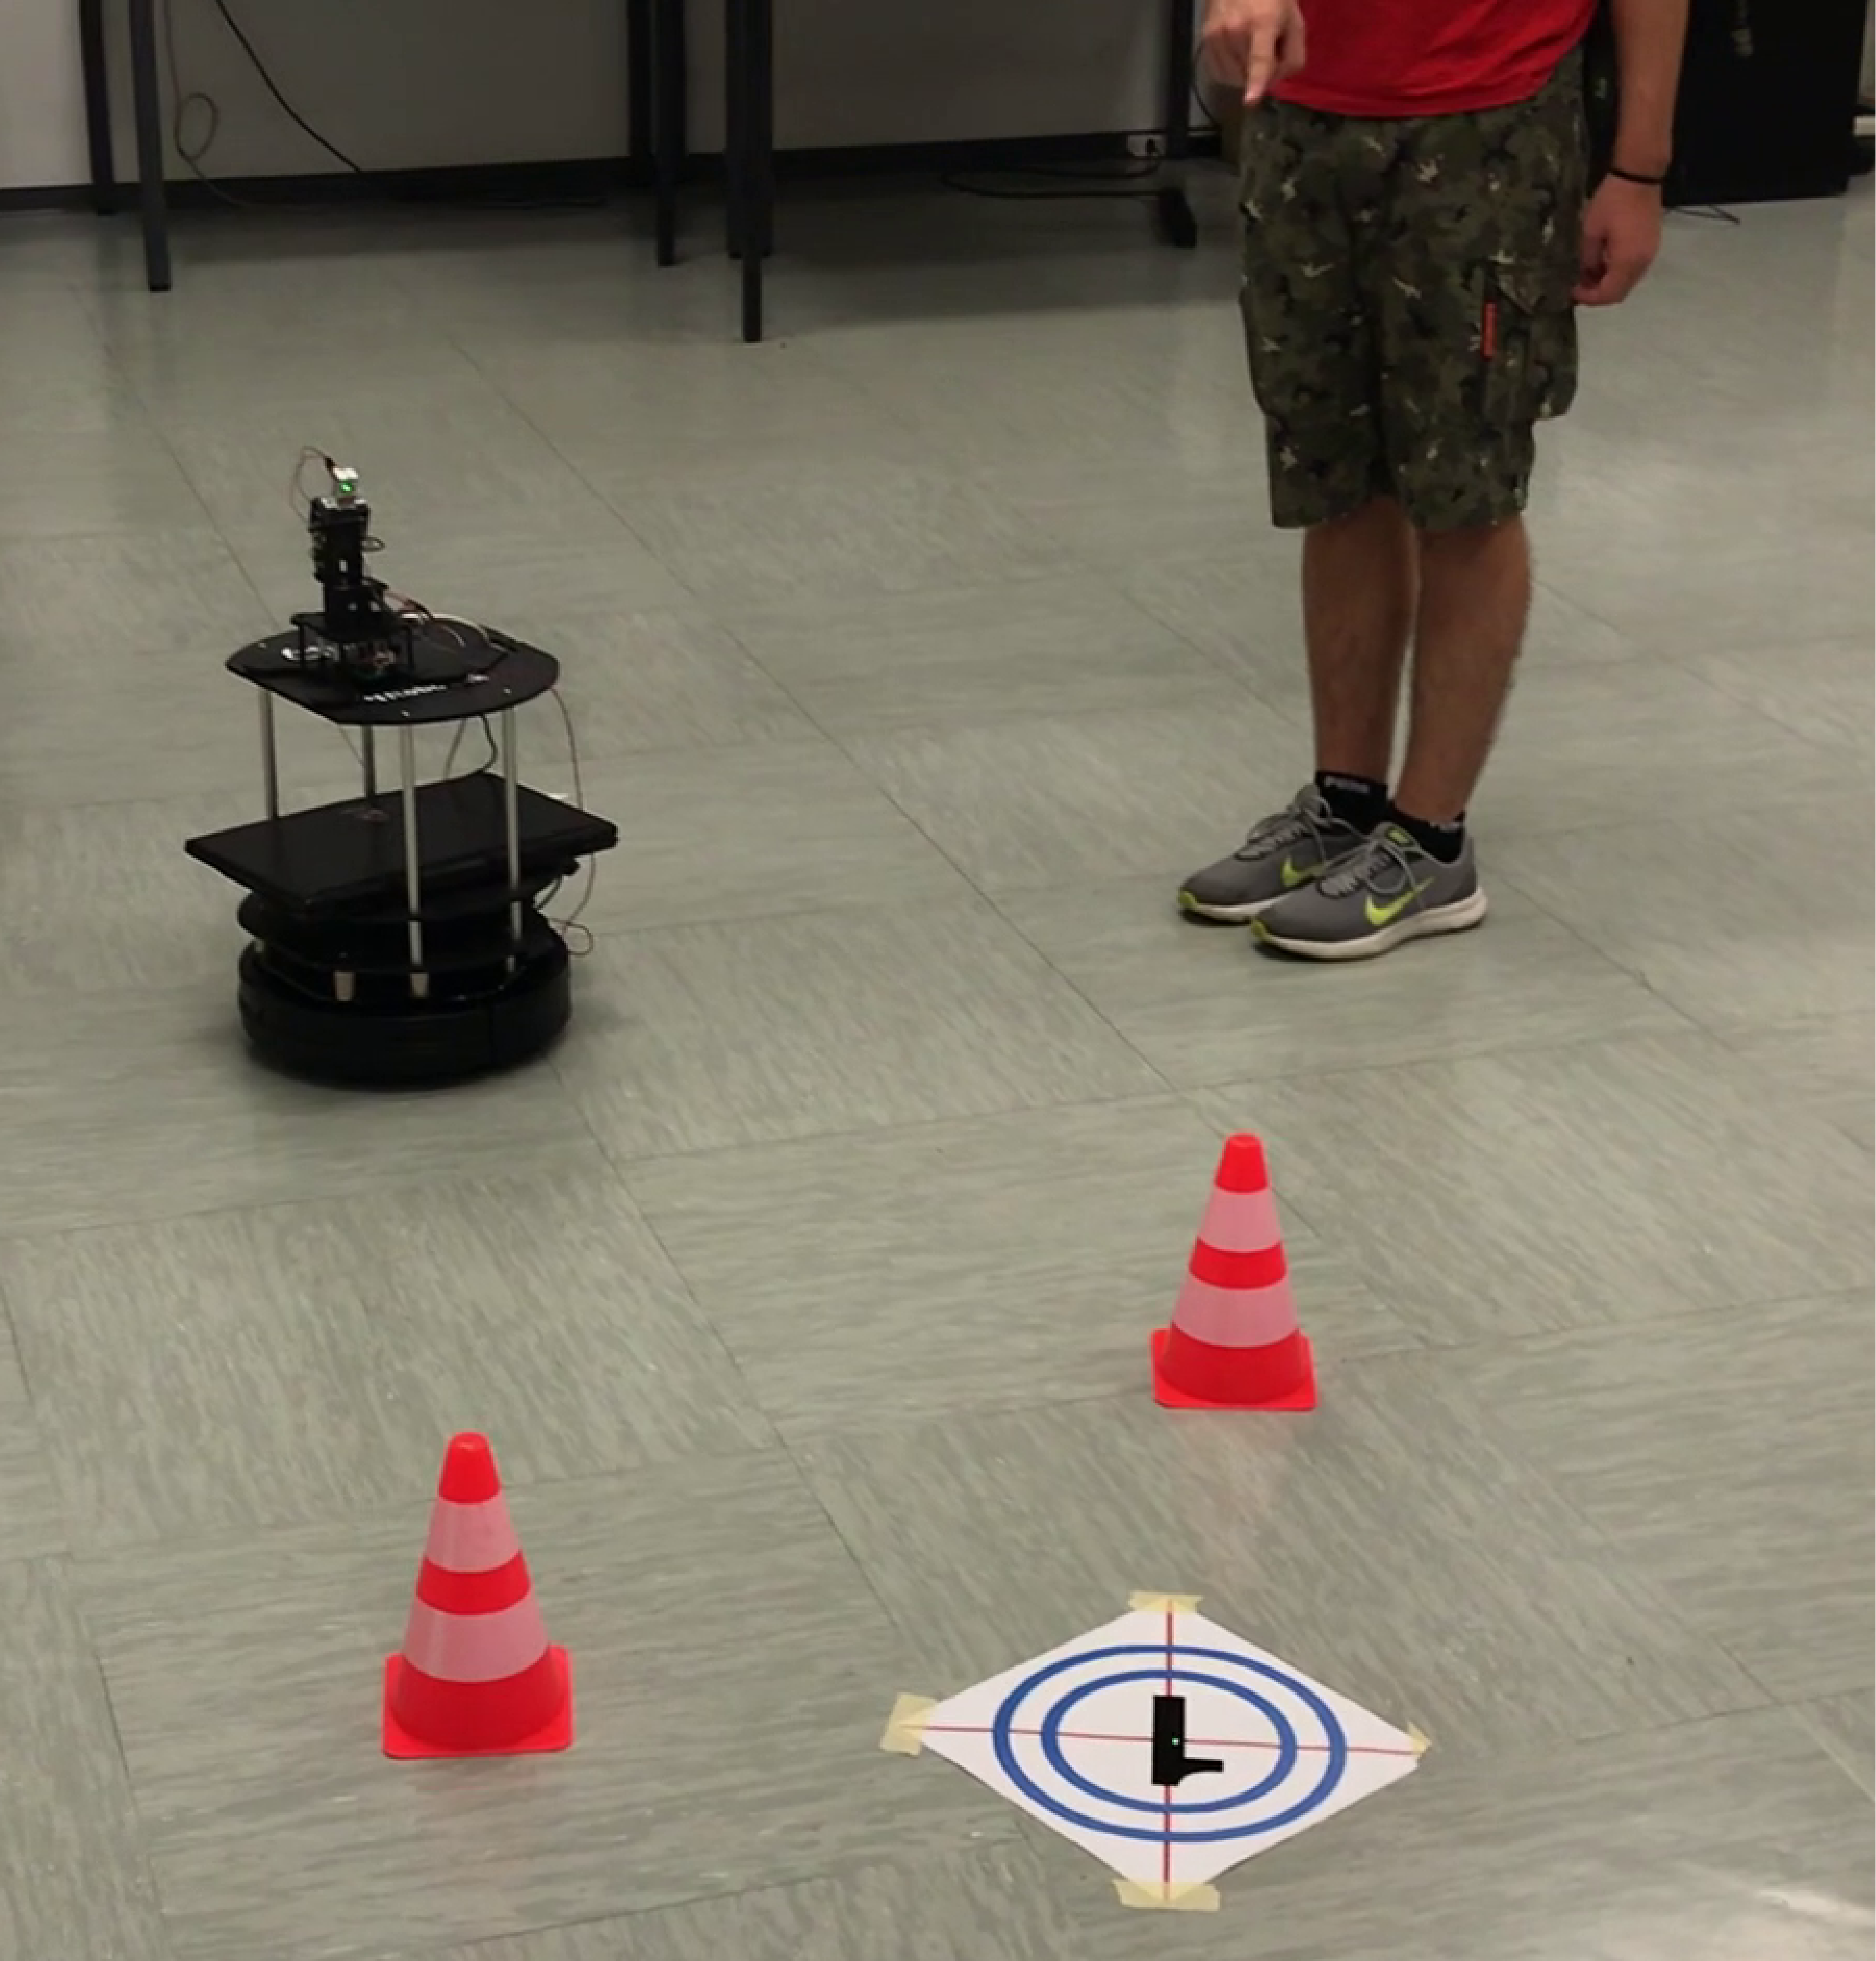
\includegraphics[width=\textwidth]{img/goToGoalDemo.png}%
	\caption{Kobuki Go to Goal Demo}
	\label{fig:goToGoalDemo}
\end{figure}
\subsection{Kobuki Follow Trajectory Demo}
In that case we have the same ingredients of the \emph{Go to Goal Demo}, but the last part is different. Now the kobuki will not simply go to a goal point, but rather it will follow a trajectory drawn by the user.\\
To mark the begin of the trajectory, the user points the start point for three seconds. After an audio feedback, he draws the trajectory with pointing gestures and finally marks the end of it again with another three seconds pointing.\\
The three second pointing detection code is the same explained in \ref{subs:kobukiGoToGoal}. Moreover, we added code to sample the trajectory point list based on distance: that means that the actual trajectory followed by the kobuki is composed of points which are at a threshold distance from their predecessor. Of course, if that threshold is zero, we are using all the sampled points.\\

\begin{figure}
	\centering
	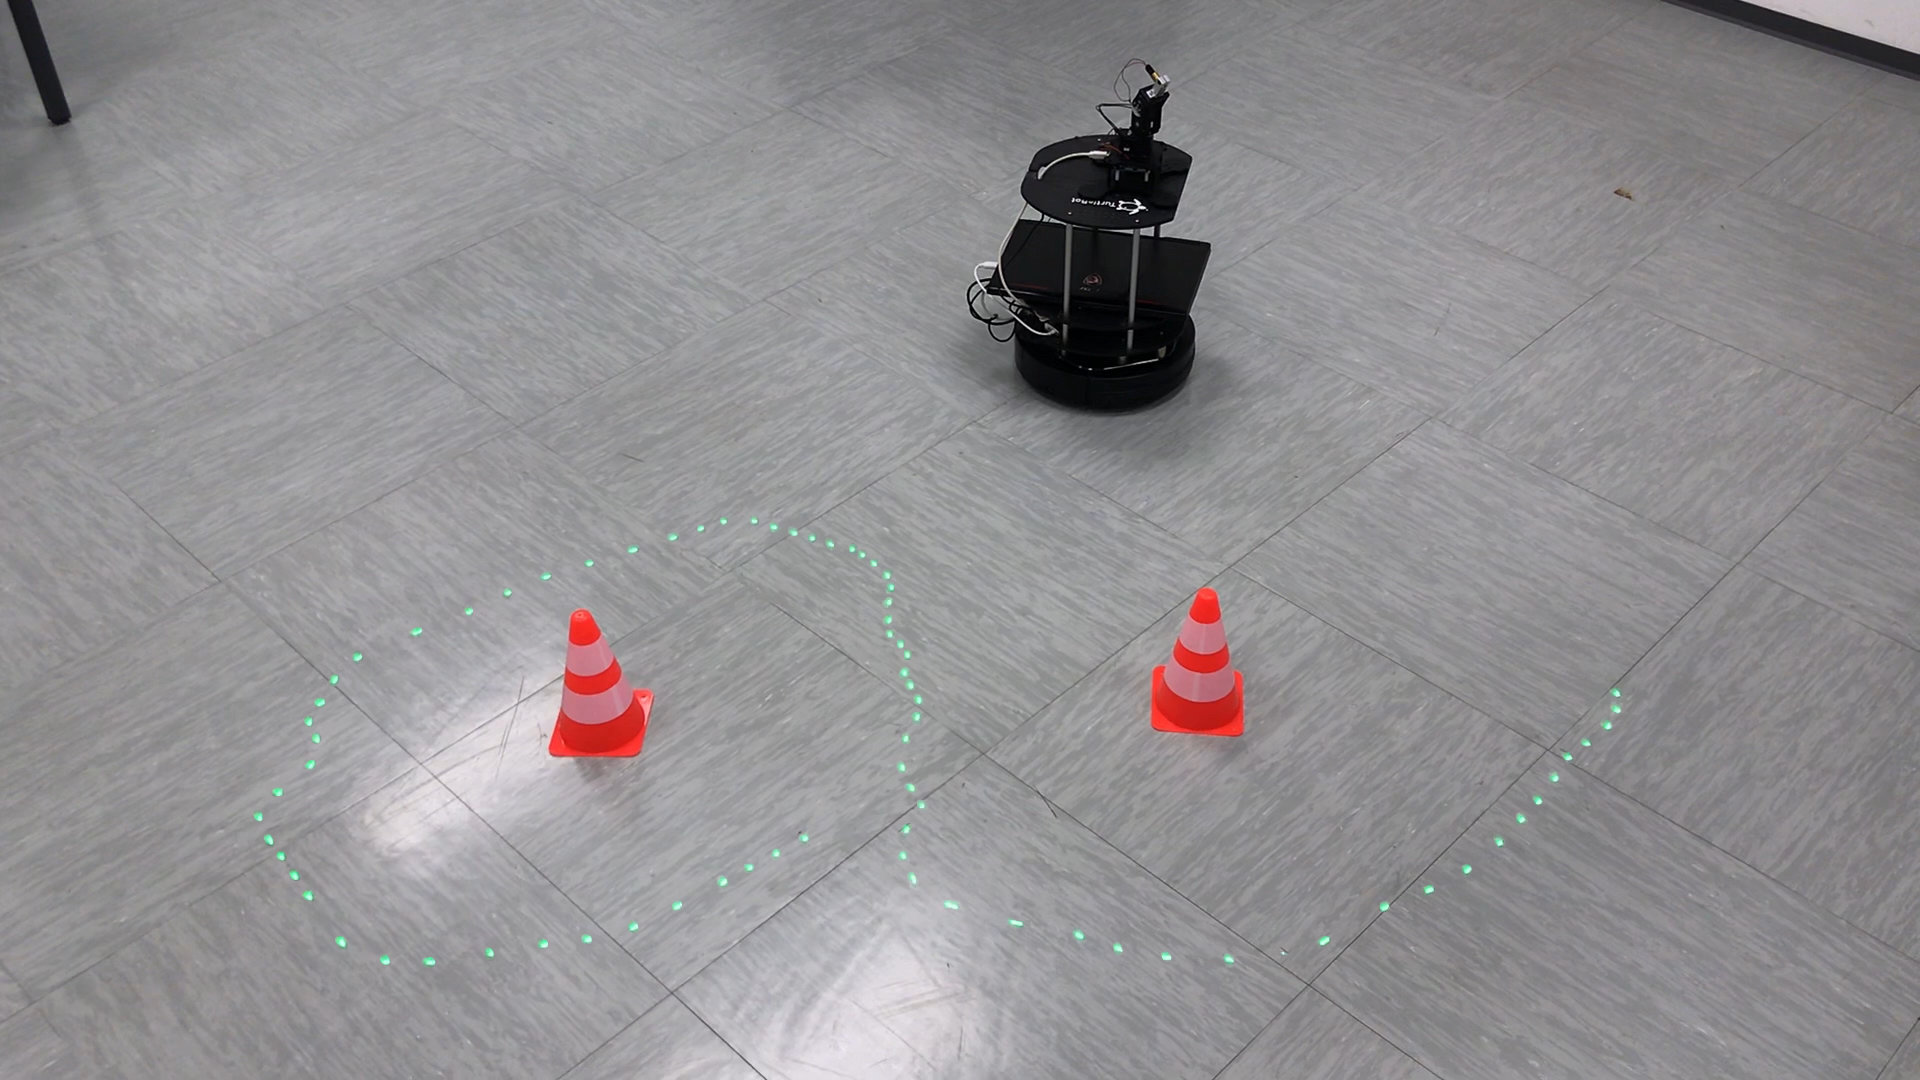
\includegraphics[width=\textwidth]{img/followTrajectoryDemo.png}%
	\caption{Kobuki Follow Trajecotry Demo}
	\label{fig:followTrajectoryDemo}
\end{figure}
